\documentclass[border=10pt]{standalone}
\usepackage{tikz}
\usetikzlibrary{shapes.geometric, arrows.meta, positioning, calc, fit, backgrounds}

\begin{document}
\begin{tikzpicture}[
    font=\sffamily,
    >=Stealth,
    node distance=1.4cm and 1.6cm,
    block/.style={draw=purple!70!black, fill=purple!8, line width=1.2pt, rounded corners=4pt, text centered, inner sep=6pt},
    reg/.style={draw=gray!80, fill=gray!20, line width=1pt, rounded corners=2pt, minimum height=2.2cm, minimum width=0.5cm, inner sep=2pt, text centered},
    bus/.style={line width=1.3pt, ->}
]

    % Input
    \node (min) at (0, 2) {\textbf{Accumulated $M$}\\ \small 4 $\times$ 4 INT36 (Signed)};

    % 1D Col Transform
    \node[block, minimum width=3.8cm, minimum height=2.8cm, right=1.4cm of min] (col_trans) {
        \textbf{4 $\times$ 1D Col Transforms}\\
        \textbf{\texttt{output\_transform\_1d}}\\
        \vspace{0.15cm}
        \small $P = A^T \cdot M$\\
        \footnotesize $p_0 = m_0 + m_1 + m_2$\\
        \footnotesize $p_1 = m_1 - m_2 - m_3$\\
        \vspace{0.1cm}
        \footnotesize Dim: $4 \times 4 \to 2 \times 4$ (38b)
    };

    % Pipeline Reg Stage 1
    \node[reg, right=1.0cm of col_trans] (reg1) {\rotatebox{90}{\textbf{REG STAGE 1 (38b)}}};

    % Transpose
    \node[block, fill=orange!8, draw=orange!70!black, minimum width=2.2cm, minimum height=2.4cm, right=1.0cm of reg1] (transp) {
        \textbf{Transpose}\\
        \vspace{0.15cm}
        \small $P^T$\\
        \footnotesize Bus rewiring\\
        \footnotesize $2 \times 4 \to 4 \times 2$
    };

    % 1D Row Transform
    \node[block, minimum width=3.8cm, minimum height=2.8cm, right=1.0cm of transp] (row_trans) {
        \textbf{2 $\times$ 1D Row Transforms}\\
        \textbf{\texttt{output\_transform\_1d}}\\
        \vspace{0.15cm}
        \small $Y' = A^T \cdot P^T$\\
        \footnotesize $y'_0 = p'_0 + p'_1 + p'_2$\\
        \footnotesize $y'_1 = p'_1 - p'_2 - p'_3$\\
        \vspace{0.1cm}
        \footnotesize Dim: $4 \times 2 \to 2 \times 2$ (40b)
    };

    % Scaling & Saturation
    \node[block, fill=red!8, draw=red!70!black, minimum width=3.2cm, minimum height=2.8cm, right=1.0cm of row_trans] (sat_block) {
        \textbf{Scaling \& Saturation}\\
        \vspace{0.15cm}
        \footnotesize Arithmetic Right Shift:\\
        \small \texttt{>>> 6} ($1/64$ scale factor)\\
        \vspace{0.1cm}
        \footnotesize Clamp to Signed INT16:\\
        \small $[-32768, +32767]$
    };

    % Pipeline Reg Stage 2
    \node[reg, right=1.0cm of sat_block] (reg2) {\rotatebox{90}{\textbf{REG STAGE 2 (16b)}}};

    % Output
    \node[right=1.2cm of reg2] (yout) {\textbf{Output Tile $Y$}\\ \small 2 $\times$ 2 INT16\\ \small \texttt{out\_valid}};

    % Busses
    \draw[bus] (min) -- node[above, font=\footnotesize] {16 $\times$ 36b} (col_trans.west);
    \draw[bus] (col_trans.east) -- node[above, font=\footnotesize] {8 $\times$ 38b} (reg1.west);
    \draw[bus] (reg1.east) -- (transp.west);
    \draw[bus] (transp.east) -- node[above, font=\footnotesize] {8 $\times$ 38b} (row_trans.west);
    \draw[bus] (row_trans.east) -- node[above, font=\footnotesize] {4 $\times$ 40b} (sat_block.west);
    \draw[bus] (sat_block.east) -- node[above, font=\footnotesize] {4 $\times$ 16b} (reg2.west);
    \draw[bus] (reg2.east) -- node[above, font=\footnotesize] {4 $\times$ 16b} (yout.west);

    \begin{scope}[on background layer]
        \node[draw=purple!50, fill=purple!2, dashed, line width=1.4pt, rounded corners=6pt,
              fit=(col_trans) (reg1) (transp) (row_trans) (sat_block) (reg2),
              inner sep=14pt,
              label={[font=\bfseries\color{purple!80!black}, anchor=north west]north west:Multiplierless 2D Output Transform Unit (\texttt{output\_transform\_2d.sv})}] {};
    \end{scope}

\end{tikzpicture}
\end{document}
